
\section{mass continuity}

\begin{frame}{the most basic shallow assumption}

\begin{columns}

\begin{column}{0.6\textwidth}
\begin{itemize}
\item there are many shallow theories: SIA, SSA, hybrids, Blatter, \dots
\item \emph{all} make one assumption not required in Stokes:

\begin{center}
\alert{the surface and base of the ice are given by functions $z=h(t,x,y)$ and $z=b(t,x,y)$}
\end{center}
\item surface overhang is not allowed
\item (and most Stokes models make this assumption too)
\end{itemize}
\end{column}

\begin{column}{0.4\textwidth}
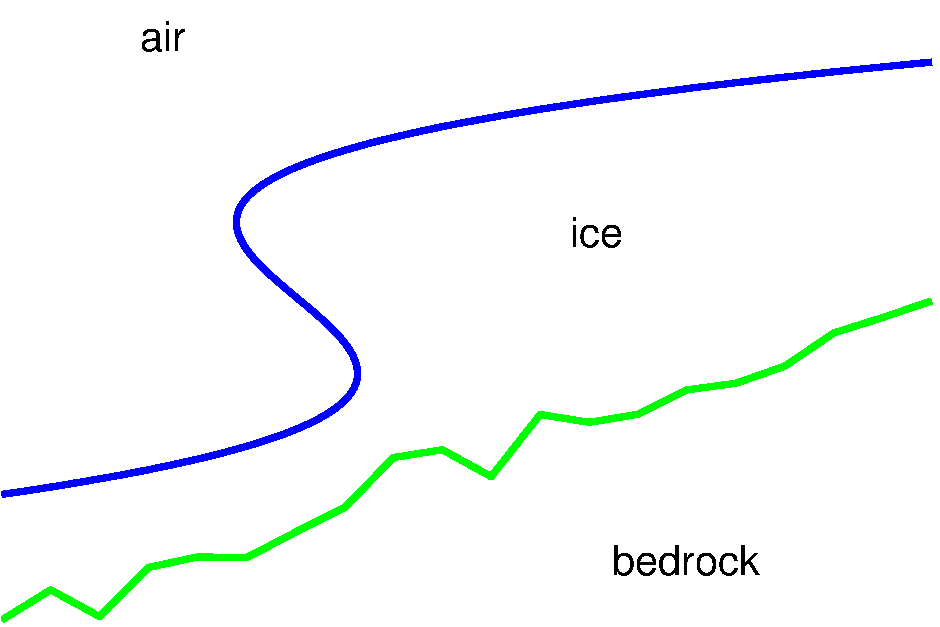
\includegraphics[width=1.0\textwidth]{sshape}

\scriptsize
\begin{center}
\emph{not shallow!}
\end{center}
\vspace{6mm}

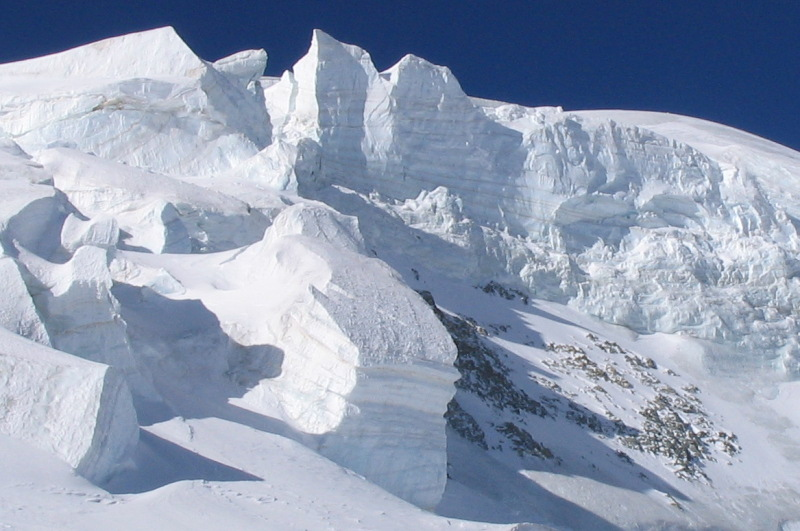
\includegraphics[width=1.0\textwidth]{serac}

\begin{center}
\emph{not shallow!}
\end{center}
\end{column}
\end{columns}
\end{frame}


\begin{frame}{three equations for geometry change}

\begin{itemize}
\item let $a$ be the climatic (surface) mass balance function;  $a>0$ is accumulation
\item $s$ be the basal melt rate function;  $s>0$ is basal melting
\item let $M=a-s$: ``climatic-basal mass balance function'' in glossary
\item define the map-plane flux of ice,
	$$\bq = \int_{b}^{h} (u,v)\,dz = \overline{\mathbf{U}}\,H$$
\item the three equations for geometry change:
\begin{align*}
&\text{surface kinematical} && h_t = a - u\big|_h h_x - v\big|_h h_y + w\big|_h  \\
&\text{base kinematical} && b_t = s - u\big|_b b_x - v\big|_b b_y + w\big|_b  \\
&\text{mass continuity} && H_t = M - \Div \bq \\
\end{align*}
\end{itemize}
\end{frame}


\begin{frame}{kinematic and mass continuity equations}

\begin{itemize}
\item what does the ``most basic shallow assumption'' get you?
\item \emph{answer}: of these three equations,
  \begin{itemize}
  \item[$\circ$]  surface kinematical
  \item[$\circ$]  base kinematical
  \item[$\circ$]  mass continuity
  \end{itemize}
\emph{any two imply the third}

\bigskip
\item to show the above, recall:
  \begin{itemize}
  \item[$\circ$]  the incompressibility of ice
    $$u_x + v_y + w_z = 0$$
  \item[$\circ$]  and the Leibniz rule for differentiating integrals
  \scriptsize
    $$\frac{d}{dx}\left(\int_{g(x)}^{f(x)} h(x,y)\,dy\right) = f'(x) h(x,f(x)) - g'(x) h(x,g(x)) + \int_{g(x)}^{f(x)} h_x(x,y)\,dy$$
  \end{itemize}
\end{itemize}
\end{frame}


\begin{frame}{kinematic and mass continuity equations 2}

\begin{itemize}
\item literature is full of incomplete calculations of these equivalences
\item \dots usually mixed in with small-parameter arguments about shallowness
\item most ice sheet models use the mass continuity equation
\item \dots but they could instead use the surface kinematical equation
\end{itemize}
\end{frame}


\begin{frame}{standard recipe for ice sheet models}

\begin{itemize}
\item the ingredients of a typical ice sheet model:
  \begin{enumerate}
  \item numerical implementation of a stress balance: compute velocity $(u,v,w)$
  \item from the horizontal velocity $(u,v)$ and the surface balance, do time-step of mass continuity equation to get $H_t$
  \item update surface elevation
  \item decide on time-step from size of diffusivity $D$, and repeat at 1.
  \end{enumerate}
\end{itemize}
\end{frame}


\begin{frame}{the mass continuity equation: a summary}

\begin{itemize}
\item the \emph{mass continuity equation} is
  $$H_t = M - \nabla \cdot (\mathbf{u} H)$$
\item the numerical nature of this equation depends on the stress balance:
  \begin{itemize}
  \item[$\circ$] the equation is a diffusion for frozen bed, large scale flows (i.e.~SIA)
  \item[$\circ$] it is \emph{not} very diffusive for membrane stresses and no basal resistance (e.g.~SSA for ice shelves)
  \item[$\circ$] it is diffusive for ice streams (but how much?)
  \item[$\circ$] there is \emph{not} much helpful theory on this transport problem
  \item[$\circ$] \dots maybe you will help find this theory!
  \end{itemize}
\end{itemize}
\end{frame}
